%!TEX root = ../physical-olympics-2.tex
\chapter{光学仪器知识摘要}


我们暂时不讨论光的干涉与衍射,\,故暂时不太需要光的波动理论.\,但实际上到了实用的层面上,\,各个光学仪器,\,从原理上说尽管几乎只用到几何光学的内容,\,似乎也是避不开对光的强度的讨论的.\,故本章先对在光的波动学说成型之前就已经蓬勃发展起来的\emph{光度学}(photometry)进行说明.\,然后从若干方面对实用频率最高的一些光学仪器做未免以偏概全的介绍.



\section{光度学}


光源产生的光,\,在光学系统中可能被光学仪器最终接收,\,如\emph{光电二极管}(photodiode),\,\emph{电荷耦合元件}(charge-coupled device,\,CCD)等.\,也可以直接被人眼所直接观察.\,很明显,\,不同仪器作为探测仪器用时,\,其光谱响应将存在很大的区别.\,然而,\,既然是光学,\,从古到今仪器的设计都是围绕人的视觉展开.\,即最核心的波段是可见光波段.\,只是,\,随着科技的发展,\,眼睛的作用逐渐被物理仪器所替代,\,对光的探测也逐渐融入了更大范围的对电磁辐射的探测中,\,后者即\emph{辐射度量学}(radiometry).\,比如当今天体物理中用到的各种探测手段,\,从波长最长的关于宇宙微波背景的射电探测,\,到波长最短的中子星$\gamma$射线暴的探测,\,俨然不再是古人仰观星空可以达到的广度和深度.\,辐射度量学以能量作为最基本的物理量进行测量,\,单位就是焦耳,\,$\mathrm{J}$.\,但是如果是考虑日常生活中以人眼视觉为核心设计的各类照明,\,媒体灯光,\,红外线,\,紫外线以外的波段几乎就被我们排除在外.\,在此之前我们需要先对人眼的独特的色视觉做一个了解:

\subsection{色视觉}
\begin{wrapfigure}[10]{o}[-10pt]{8cm}
\centering
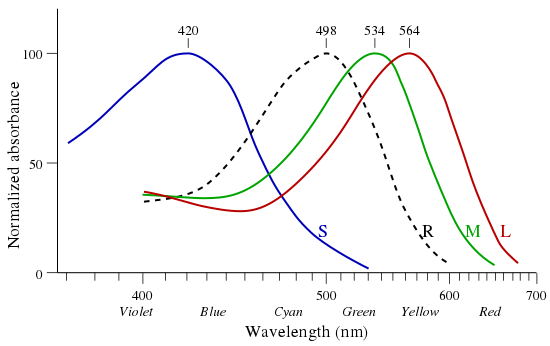
\includegraphics[width=8cm]{image/5-8-1.png}
\caption{四钟感光细胞相对响应}
\end{wrapfigure}
大部分人类的视网膜内有两种大类的视觉感受细胞:\,\emph{视锥细胞}(cone)与\emph{视杆细胞}(rod).\,而视锥细胞又根据其所含视蛋白质分为感受$500-700\mathrm{nm}$波长的\emph{视红素}细胞(protan,\,erythrolabe,\,L,\,$\rho$);\,感受$450-630\mathrm{nm}$波长的\emph{视绿素}细胞(deutan,\,chlorolabe,\,M,\,$\gamma$)和感受$400-500\mathrm{nm}$波长的\emph{视蓝素}细胞(tritan,\,cyanolabe,\,S,\,$\beta$)\footnote{在女性中常见异常X染色体导致个体产生四种色素的视锥细胞从而其色视觉明显优于一般的男性或女性}.\,




\section{光阑与光瞳}

\section{眼睛}

\section{显微镜}

\section{望远镜}

\section{照相机}